\documentclass[12pt]{article}
\usepackage{graphicx}
%\title{IF\_curr\_comb\_exp: combined exponential synaptic response}
\title{Synapse Modelling on SpiNNaker}
\author{Oliver Rhodes}
\date{\today}


\begin{document}
\maketitle

\begin{abstract}
This article introduces the various types of synapse model available within the
current SpiNNaker API, and then discusses several extensions and new models to
cover methods from the literature on computational neuroscience. The underlying
models, together with SpiNNaker-specific implementation details are discussed,
followed by a comparison of the effects on wider neural networks.
\end{abstract}

\section{Introduction}
In neuron-based modelling, neural networks are defined from populations of
neurons, and then connected via synapses, replicating the physiological layout
of the brain. The neurons take input from others in the network when connected
neurons spike, leading to a transfer of current from synaptic binding. The
neuron behaviour -- such as firing dynamics and threshold -- are typically
defined by a neuron model: with common implementations including the leaky
integrate and fire (LIF) ***cite***, or Izhikevich ***cite*** neurons. These
essentially govern how and when a neuron will fire, and once fired, the reset
state. How these neurons are excited and inhibited by others in the
network is determined by the firing of connected neurons. Upon firing a
presynaptic neuron will cause binding of the synaptic transmitters, which in
turn open ion channels, allowing current to flow. This flow of current is fed
into the post-synaptic neuron, causing a resulting effect in the neuron model.

The time-dependent behaviour of this synaptic response (i.e. what current
is fed into the post-synaptic neuron) is the subject of the remainder of this
work: in the following section various synaptic model are introducted, before
results are presented for comparion and dicussion.

\section{Synapse Modelling}
Due to the high connectivity between neurons in the brain, sysnapses form a
major part of neural netowrks. Their number can exceed the number of neurons by
several orders of magnitude ***cite***, meaning efficient implementation is a
critical factor in overall network performance ***cite***. Further consideration
must also be made of the underlying computational framework used to build and
run the neuralnetwork. In this work the SpiNNaker platform is used, which
presents various restrictions ***cite*** such as: limited memory (for both
instruction ITCM, and state variables DTCM), and 32-bit fixed-point arithmetic
without division support. This section covers the introduction of four models,
representing increasing complexity and computational cost. For each model, the
underlying mathematical response is introduced, followed by details of the
SpiNNaker-specific implementation.

\subsection{Instantaneous Rise and Exponential Decay}
\subsubsection*{Synaptic Response}
The response of ion channels opening and closing is typcially characterised by
fast opening, followed by slower closing ***cite***. As the charge flowing
through the synapse is proportional to this opening and closing, a simple and
efficient response can be defined using an instanaeous rise to peak flow (upon
the presynaptic neuron receiving a spike), followed by an exponential decay
back to a closed state. Modelling using exponential function, the conductance
as a function of time $g(t)$, is defined mathematically as:
\begin{equation}
g(t) = \bar{g}_{syn} e^{-t/\tau}
\end{equation}
where $t$ is time, and $\tau$ is a decay constant governing rate of closing of a
synapse.

\subsubsection*{SpiNNaker Implementation}
Because of the lack of division operator on SpiNNaker, the quotient $t/\tau$ is
precomputed, and a multiplier used to decay the conductance by a consistent
fraction over each timestep. For example, if $\tau = 5$, and the simulation
timestep is $\delta t = 0.1 \mathrm{ms}$, this factor is given by $e^{t/\tau} =
e^{0.1/5} = 0.980$
The code to evaluate synapse shaping therefore requires parameters for: the
decay scalar, the initial decay scalar, and the current value of the evaluated
exponential (for use by the postsynaptic neuron). To enable fixed-point
computation of output values, each parameter is stored via a custom SpiNNaker
datatype occupying

\subsection{Alpha Response}
The alpha response represents a more physiologically-accurate synaptic response,
whereby the synaptic ion channels open over a finite time interval. The
response is typically comprised of a fast opening time, and hence initial rise
in conductance, followed by a relatively slow decay back to the closed state (see
Fig.~ ***)

\subsubsection*{Synaptic Response}
The characteristic `alpha' response is defined by two coupled differential
equations.  Upon combination, and setting equal time constants, a response
similar to combining two exponential responses is achieved. The response of
$g_{syn}$, together with the two coupled differential equations, can be defined
as:
\begin{eqnarray}
g_{syn}(t) & = & \bar{g}_{syn}fg(t) \nonumber \\
\frac{dg}{dt} & = & \frac{1}{\tau_{decay}} (-g + h) \nonumber \\
\frac{dh}{dt} & = & \frac{1}{\tau_{rise}}(-h) \nonumber
\label{eqn:alpha_coupled_diff_eqns}
\end{eqnarray}

Setting $\tau_{rise}=\tau_{decay} = \tau$ and solving for $h(t)$ via separation
of variables:
\begin{eqnarray}
\int \frac{1}{h} dh & = & \int -\frac{1}{\tau}dt \nonumber \\
\ln{h}&=&-\frac{t}{\tau} + C \nonumber \\
h(t) & = & e^{-{t/\tau}+C} = ke^{-t / \tau} \nonumber
\label{eqn:solve_for_h}
\end{eqnarray}
Rearranging to the form $\frac{dy}{dt} +Py = Qt$, substituting  for $h(t)$, and
solving for $g(t)$ by integration via the particular integral (and the reverse
product rule):
\begin{eqnarray}
\frac{dg}{dt} + \frac{g}{\tau}&=&\frac{k}{\tau}e^{-t/\tau} \nonumber\\
\mathrm{P.I.}&=& e^{\int P dt} = e^{t/ \tau} \nonumber \\
e^{t/\tau}\frac{dg}{dt} + e^{t/\tau}\frac{g}{\tau}
&=& \frac{k}{\tau}e^{-t/\tau}e^{t/\tau} \nonumber \\
\frac{d}{dt} g e^{\frac{t}{\tau}}&=&\frac{k}{\tau}e^{-\frac{t}{\tau}
+\frac{t}{\tau}} \nonumber \\
g e^{\frac{t}{\tau}} &=& \int \frac{k}{\tau}e^0 dt  =  \frac{kt}{\tau} \nonumber \\
g(t)&=&\frac{kt}{\tau}e^{-t/\tau}
\end{eqnarray}


\subsubsection*{SpiNNaker Implementation}

\subsection{Combined Exponentials}
\subsubsection*{Synaptic Response}
Whilst the alpha synapse offers flexibility to define a range of fast rising and
slowly decaying conductance profiles, the two regimes are inherentyl coupled,
and hence it's difficult to effect the individual rise and decay components of
the overall response. To overcome this limitation, and to faciliate
an instantaneous rise and two-phase decay respone, a conductance profile based
on the combination of two exponentials is defined below.

The response is built from the summation of two exponential decay functions,
similar to that defined for the instantaneous rise and decay model. However, in
this general implementation, coefficients $A$ and $B$ are added to enable
scaling of the individual components. The conductance profile can therefore be
defined as:
\begin{equation}
g_{syn}(t)=\bar{g}_{syn}f\Big(Ae^{-t / \tau_a} + Be^{-t / \tau_b}\Big)
\label{eqn:combined_general_form}
\end{equation}
where $\tau_a$ and $\tau_b$ define two individual time constants. The response
in Eqn.~\ref{eqn:combined_general_form} faciliates two interesting behaviours
when the signs of constants $A$ and $B$ are either equal or opposite.

\paragraph{Difference of two exponentials: $A>0, B<0$}
Setting the coefficients $A = -B = 1$, together with $\tau_a = $
\
\begin{eqnarray}
t_{rise}&=&ln\frac{B\tau_x}{A\tau_x}\frac{\tau_x\tau_x}{\tau_x - \tau_x} \\
f&=&\Big( e^{-t_{rise} / \tau_a} - e^{-t_{rise} / \tau_b}\Big)^{-1}
\label{eqn:combined_exponential_response}
\end{eqnarray}
\begin{figure}[!h]
\begin{centering}
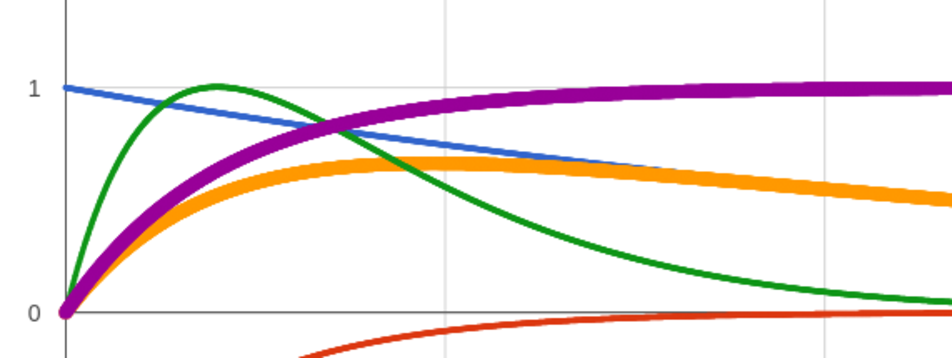
\includegraphics[width=0.5\textwidth]{combined_general_difference.ps}
\caption{Example conductance response for combined exponential model}
\label{fig:combined_exp_example}
\end{centering}
\end{figure}

\paragraph{Cumulation of two exponentials: $A>0, B>0$}
\begin{figure}[!h]
\begin{centering}
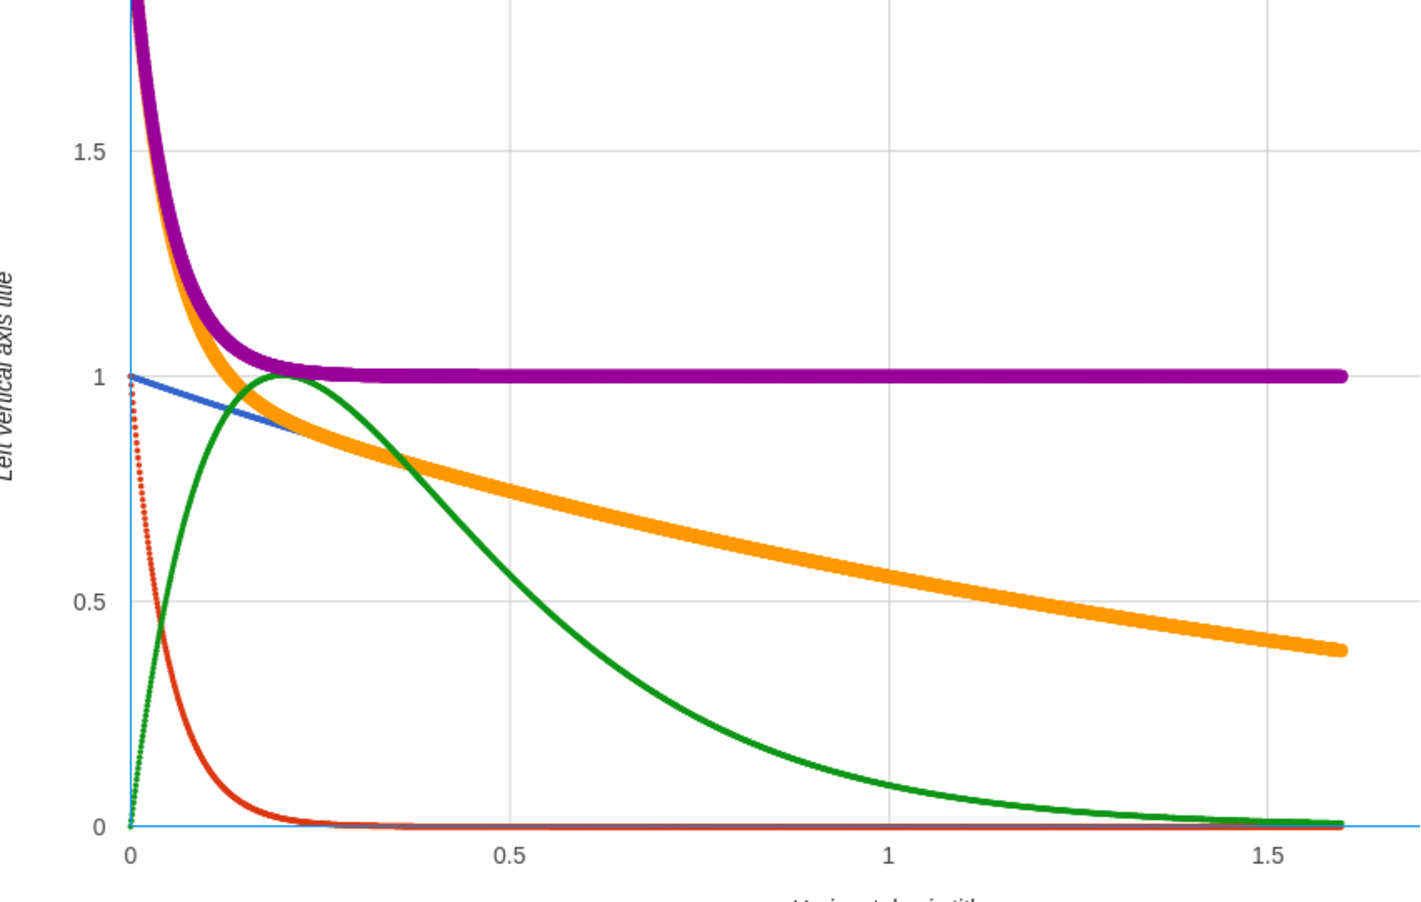
\includegraphics[width=0.5\textwidth]{combined_general_cumulation.ps}
\caption{Example conductance response from summation of two exponential
components}
\label{fig:combined_exp_example}
\end{centering}
\end{figure}

\subsubsection*{SpiNNaker Implementation}
A generic combined exponential synapse is implemented to facilitate exploration
of further synapse shapes defined through combinations of exopnential
functions. The conductance $g_{syn}(t)$ is therefore defined as in
Eqn.\ref{eqn:combined_general_form}.

To give the respone defined in Eqn.~\ref{eqn:combined_exponential_response},
coefficients are set $A=-B=f$. The response defined in ***cite*** can then be
repeated by setting $\tau_a = \tau_{rise} = 1.7$ and $\tau_b = \tau_{decay} =
0.2$. These coefficients give the response shown in Fig.~\ref{fig:typical_response}.
\begin{figure}
\caption{Synapse behaviour replicating ***cite***, achieved through combining
exponetnials according to \ref{eqn:combined_general_form} and setting coefficients
$A=-B=f$ (where $f$ is calculated according to Eqn.~\ref{eqn:combined_exponential_response}), and $\tau_a = 1.7$ and $\tau_b = 0.2$.}
\label{fig:typical_response}
\end{figure}
Note that Fig.~\ref{fig:typical_response} also shows the two components before
combining: this shows that for the coefficients given, the early response is
dominated by the contribution from the first component -- designated
$\tau_{rise}$ -- with the subsequent response dominated by the second component
-- designated $\tau_{decay}$.


\subsection{Biphasic}
\subsubsection*{Synaptic Response}
\subsubsection*{SpiNNaker Implementation}

\section{Results}

\section{Discussion}

\end{document}
